\documentclass[12pt]{article}
\usepackage{graphicx}
\graphicspath{ {./images/} }
\usepackage{amsthm,amssymb,amsmath,amsfonts}
\usepackage[a4paper, top=25mm, bottom=30mm, left=25mm, right=25mm]{geometry}
\usepackage[pagebackref=false,colorlinks,linkcolor=black,citecolor=black]{hyperref}
\usepackage[nameinlink]{cleveref}
 \AtBeginDocument{%
    \crefname{equation}{برابری}{equations}%
    \crefname{chapter}{فصل}{chapters}%
    \crefname{section}{بخش}{sections}%
    \crefname{appendix}{پیوست}{appendices}%
    \crefname{enumi}{مورد}{items}%
    \crefname{footnote}{زیرنویس}{footnotes}%
    \crefname{figure}{شکل}{figures}%
    \crefname{table}{جدول}{tables}%
    \crefname{theorem}{قضیه}{theorems}%
    \crefname{lemma}{لم}{lemmas}%
    \crefname{corollary}{نتیجه}{corollaries}%
    \crefname{proposition}{گزاره}{propositions}%
    \crefname{definition}{تعریف}{definitions}%
    \crefname{result}{نتیجه}{results}%
    \crefname{example}{مثال}{examples}%
    \crefname{remark}{نکته}{remarks}%
    \crefname{note}{یادداشت}{notes}%
    \crefname{observation}{مشاهده}{observations}%
    \crefname{algorithm}{الگوریتم}{algorithms}%
    \crefname{cproof}{برهان}{cproofs}%
}

\usepackage{tikz}
\usepackage{graphicx}
\usepackage{color}

\usepackage{setspace}
\doublespacing

\usepackage{titletoc}
\usepackage{tocloft}
\usepackage{enumitem}

\usepackage{algorithm}
% \usepackage[noend]{algpseudocode}
\usepackage[noend]{algorithmic}
\renewcommand{\algorithmicrequire}{\textbf{Input:}}
\renewcommand{\algorithmicensure}{\textbf{Output:}}

\usepackage{tabularx}
\makeatletter
\newcommand{\multiline}[1]{%
  \begin{tabularx}{\dimexpr\linewidth-\ALG@thistlm}[t]{@{}X@{}}
    #1
  \end{tabularx}
}
\makeatother

\usepackage{float}
\usepackage{verbatim}
\makeindex
\usepackage{sectsty}
\usepackage{xepersian}
\SepMark{-}
\settextfont[Scale=1.2,Path=fonts/,BoldFont=B Nazanin Bold.ttf]{B Nazanin.ttf}
\setlatintextfont{Times New Roman}
\renewcommand{\labelitemi}{$\bullet$}

\theoremstyle{definition}
\newtheorem{definition}{تعریف}[section]
\newtheorem{remark}[definition]{نکته}
\newtheorem{note}[definition]{یادداشت}
\newtheorem{example}[definition]{نمونه}
\newtheorem{question}[definition]{سوال}
\newtheorem{remember}[definition]{یاداوری}
\newtheorem{observation}[definition]{مشاهده}
\theoremstyle{theorem}
\newtheorem{theorem}[definition]{قضیه}
\newtheorem{lemma}[definition]{لم}
\newtheorem{proposition}[definition]{گزاره}
\newtheorem{corollary}[definition]{نتیجه}
\newtheorem*{cproof}{برهان}




\begin{document}
\fontsize{12pt}{14pt}\selectfont
\begin{minipage}{0.1\textwidth}

\end{minipage}%
\hfill%
\begin{minipage}{0.6\textwidth}\centering
\fontsize{10pt}{10pt}\selectfont
به نام خداوند \\
تئوری یادگیری ماشین \\
دکتر سیدصالحی\\
جلسه سوم
 \\
\vspace{0.25cm}
\begingroup
\fontsize{8pt}{8pt}\selectfont
دانشکده ریاضی و علوم کامپیوتر \\
اسفند ماه 1402\\
\endgroup
\end{minipage}%
\hfill%
\begin{minipage}{0.1\textwidth}
\end{minipage}

\vspace{0.5cm}

\noindent\rule{\textwidth}{1pt}

\section*{مسئله یادگیری $supervised$}
اکنون یک نمونه از مشکلات یادگیری تحت نظارت را بررسی میکنیم. فرض کنید مجموعه داده ای داریم که مناطق زندگی و قیمت 47 خانه را از تهران ارائه می دهد:

\begin{figure}[htbp]
  \centering
  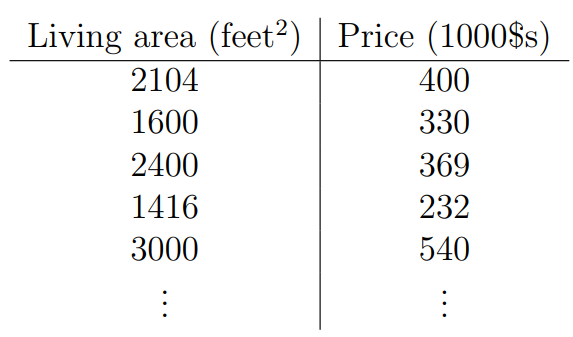
\includegraphics[width=0.4\textwidth]{etc/Images/Fig1.png} 
  \caption{داده های 47 خانه در تهران}
  \label{fig1}
\end{figure}

\begin{figure}[htbp]
  \centering
  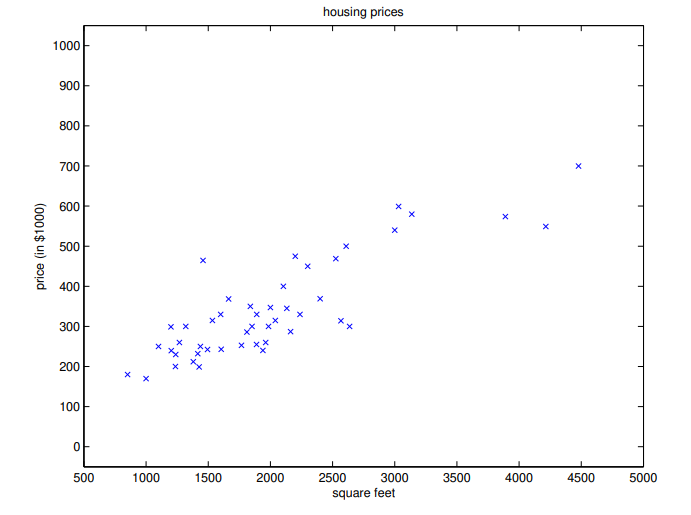
\includegraphics[width=0.4\textwidth]{etc/Images/Fig3.png} 
  \caption{داده های پلات شده}
  \label{fig3}
\end{figure}


*$h(x)$ مجموعه همه ی خط ها در فضای دو بعدی است و فضای فرضیه ساخته شده 
$h : X\longrightarrow Y$
برابر با تمام خطوط ممکن در فضای دو بعدی می باشد .

\begin{figure}[htbp]
  \centering
  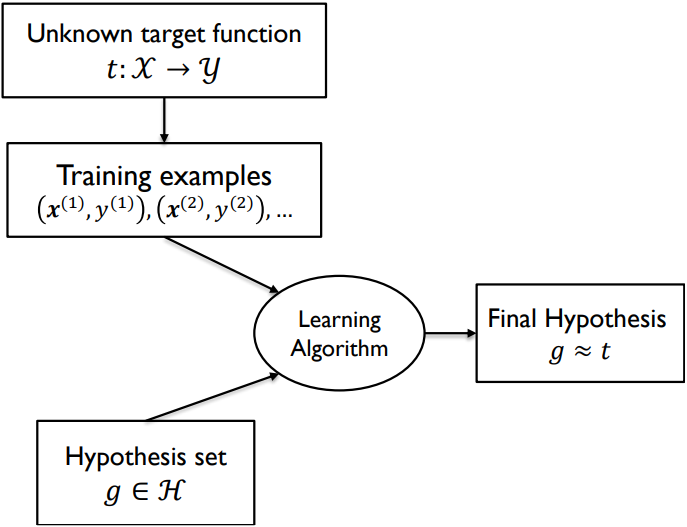
\includegraphics[width=0.4\textwidth]{etc/Images/Fig2.png} 
  \label{fig2}
\end{figure}
هنگامی که متغیر هدفی که می‌خواهیم پیش‌بینی کنیم پیوسته باشد، مانند مثال قیمت خانه های شهر، مسئله یادگیری را مسئله \textbf{رگرسیون} می‌نامیم. وقتی $y$ بتواند فقط تعداد کمی از مقادیر گسسته را به خود بگیرد و تعداد $output$ ها محدود باشد، ما آن را یک مسئله $classification$ می‌نامیم.

\subsection*{$regression$ $Linear$}
برای انجام یادگیری تحت نظارت، باید تصمیم بگیریم که چگونه فرضیه های $h$ را مدل کنیم در کامپیوتر. به عنوان یک انتخاب اولیه، فرض کنید تصمیم داریم $y$ را به عنوان تابع خطی $x$ تقریب کنیم:
\\
\[
h_w(x) = w_0 + w_1x_1 + w_2x_2
\]

جایی که $w_i$ ها پارامترها یا وزن های مدل نامیده می شوند که فضای توابع خطی نگاشت $h : X\longrightarrow Y$ را پارامتر می کنند. در اینجا $w_0$ عرض از مبدا و 
$w_1$
شیب می باشد .
\\
\\
برای ساده کردن $notation$، ما $x_0$ را 1 قرار میدهیم  معرفی می کنیم، به طوری که حاصل میشود:
\[
h(x)=\sum_{i=0}^{d}{w}_{i}x_{i}={w}^{T}x,
\]

ولی خب بدیهتا تابع ما با دیتای واقعا اختلافاتی دارد و خطاهایی موجود است که به صورت زیر میتوان اندازه گیری کردشان:
\[
loss = (y - h(x))^2
\]
حال، با توجه به یک داده های آموزشی، چگونه پارامترهای $w$ را انتخاب کنیم یا یاد بگیریم؟ به نظر می رسد یک روش معقول این است که $h(x)$ را به $y$ نزدیک کنیم، حداقل برای مثال های آموزشی که داریم. اکنون تابعی را تعریف می‌کنیم که برای هر مقدار $w$، میزان نزدیکی $h(x(i))$ به $y(i)$ مربوطه را اندازه می‌گیرد. $cost function$ را تعریف می کنیم:
\[
J(\theta)=\frac{1}{2}\sum_{i=1}^{n}(h_{\theta}(x^{(i)})-y^{(i)})^{2}
\]

\begin{figure}[htbp]
  \centering
  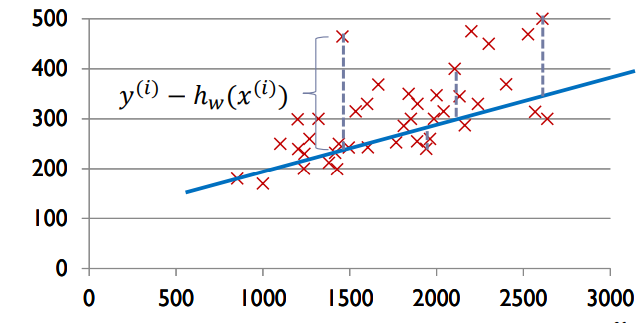
\includegraphics[width=0.5\textwidth]{etc/Images/Fig4.png} 
  \caption{یک نمایش از اینکه چگونه یک مدل خطی با مجموعه ای از داده ها مطابقت دارد.}
  \label{fig4}
\end{figure}

\subsection*{$algorithm$ $learning$  $The$}
هدف اصلی ما این است که $w$ را طوری انتخاب کنیم که $J(w)$ را به حداقل برسانیم.
 برای هر فرضیه در فضای فرضیه یک تابع هزینه در نظر میگیرم و با مینیمم کردن تابع هزینه پارامتر های بهترین فرضیه رو یاد میگیره که حل این مساله $optimization$ است.

اولین راهی که به ذهن می رسد مشتق گیری و برابر صفر قرار دادن تابع ما است یعنی : 
$$\frac{\partial J(w)}{\partial w_0} 
 = 0 $$
 $$\frac{\partial J(w)}{\partial w_1} 
 = 0 $$

  در واقع مقدار تابع گرادیان برابر صفر است و دو دستگاه معادلات خطی داریم و میتوانیم این دو را به دست آوریم .
 برای حالت 
 $multivariate$
 ماتریس در نظر می گیریم به نوعی که برای هر سمپل به اندازه ی 
 $d$
 فیچر داریم .
 هر سطر 1 سمپل را نشان می دهد 
 پس :

\begin{figure}[htbp]
  \centering
  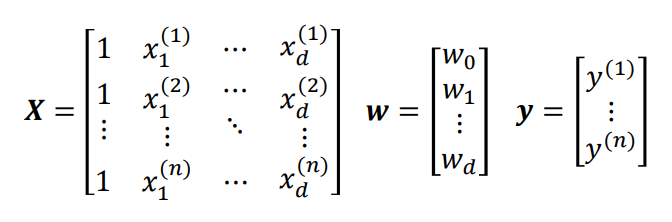
\includegraphics[width=0.50\textwidth]{etc/Images/Fig5.png} 
  \caption{ماتریس های سمپل ها، وزن ها و $y$}
  \label{fig5}
\end{figure}

که میتوان میزان هزینه را به شکل زیر بدست آورد:

\[
J(w)=\sum_{i=1}^{n}(y^{(i)}-h_{w}(x^{(i)}))^2=\sum_{i=1}^{n}(y^{(i)}-w^{T}x^{(i)})^2
\]

برای پیاده سازی این الگوریتم، باید مشخص کنیم که عبارت مشتق جزئی در سمت راست چیست. بیایید ابتدا آن را برای حالت اگر ما فقط یک مثال آموزشی داریم $(x, y)$ کار کنیم تا بتوانیم از مجموع در تعریف $J$ صرف نظر کنیم. داریم:
\begin{align*}
\frac{\partial}{\partial w_j}J(w) &= \frac{\partial}{\partial w_j} (h_w(x) - y)^2 \\
&= 2 (h_w(x) - y) . \frac{\partial}{\partial w_j}(h_w(x) - y)^2 \\
&= 2 (h_w(x) - y)^2  . \frac{\partial}{\partial w_j} \left(\sum_{i=1}^{d} w_i x_i - y \right)
\\
&=2 (h_w(x) - y) x_i
\end{align*}

مشتق تابع هزینه را با توجه به $w$ ها را صفر قرار دهید.
\begin{figure}[htbp]
  \centering
  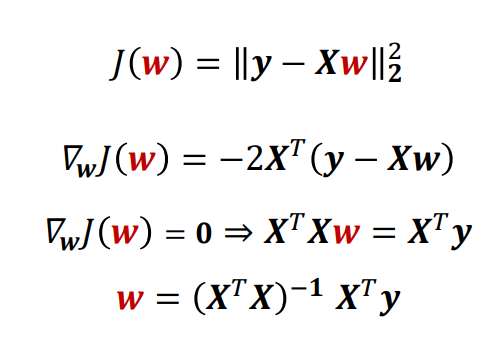
\includegraphics[width=0.4\textwidth]{etc/Images/Fig6.png} 
  \label{fig6}
\end{figure}

چرا 
$X^TX $
وارون پذیر است ؟

ماتریس سمپل $X$ ها فول رنک می باشد و وارون پذیر است .
البته با چالش هایی نیز مواجه هستیم .





\end{document}